\section{Object Relational Mapping (ORM)}
Come sappiamo non si ha una relazione diretta tra OOP(Object Oriented Programming) e modello relazionale e per questo si usa l'\textbf{Object Relational Mapping (\textit{ORM})} quando si lavora con la OOP ma con dati persistenti in un database (con le classi che vanno mappate nelle entità e viceversa). Esistono dei framework che utilizzano implementano questa tecnica.\\
Quello che si cerca è di avere una costruzione che sia quanto più possibile trasparente, rispetto alla parte di persistenza e memorizzazione dei dati, e che ci permetta di scrivere il codice in modo coerente, riferendoci unicamente al modello Object Oriented. Molti dei concetti si applicano ad altri framework, che magari non mirano al solo Object Oriented.\\
La soluzione al ORM (quindi alla tecnica di relazionamento), dal punto di vista architetturale, prevede un Client che utilizza un Model e dati che devono rimanere persistenti su una Resource. Il problema risulta il far comunicare Client e Resource. La soluzione è data dall'inserimento di un API Gateway che ha il compito di eseguire la traduzione bilaterale della comunicazione tra i due elementi.\\
Concretamente diremo che si sfrutta un \textit{API gateway} tra il client e le risorse dati (il database in questo caso) che incapsula l'accesso a una risorsa esterna con una classe e traduce le richieste di accesso alla risorsa esterna in chiamate all'API. Con questo approccio si nasconde l'accesso alle risorse (rendendone anche facile la modifica) e la complessità delle API.
\subsection{database Gateway}
Si hanno tipicamente 4 pattern per il \textbf{database gateway}:
\begin{itemize}
    \item \textbf{Table Data Gateway}, che prevede un oggetto che funge da gateway per una determinata tabella del database. Dispone di un'interfaccia semplice, solitamente costituita da: diversi metodi di ricerca per ottenere i dati da database, metodi di update, insert e delete. Ogni metodo mappa i parametri di input in una chiamata SQL e esegue l'SQL su una connessione al database. Il Table Data Gateway è solitamente privo di stato (stateless), poiché il suo ruolo è quello di portare i dati avanti e indietro. Un problema del TDG è che anche una semplice query di ricerca tramite ID restituirà più elementi, invece che uno. In ambienti in cui puoi restituire più elementi, puoi utilizzare quelli per una singola riga, ma molti liuguaggi forniscono un solo valore di ritorno e molte query restituiscono più righe. Risulta comodo nel paradigma procedurale ma meno in quello OOP in quanto i metodi ritornano dati row e non oggetti.
    \item \textbf{Row Data Gateway}, prevede un oggetto che funge da gateway per un singolo record all'interno del data source. Prevede quindi un oggetto per record, comportando che si possono avere più copie di oggetti persistenti in memoria, avendo una classe gateway che funge da alter-ego del database che viene chiamata dalla classe coi metodi \textit{finder} (che però potrebbero essere implementati direttamente nella classe gateway).
    \item \textbf{Active Record}, che prevede un oggetto per record
    \item \textbf{Data Mapper}, che prevede un layer applicativo dedicato all'ORM
\end{itemize}
\subsubsection{Active record}
Questo pattern è una versione ottimizzata del \textit{row data gateway}.\\ Considerate le classi che implementano i dati che devono essere persistenti si arricchiscono le classi con metodi per permettere l'interazione col database. Un \textbf{active record} include quindi:
\begin{itemize}
    \item la business logic
    \item il mapping logico al database, avendo come metodi statici i \textit{metodi finder} (quelli spiegati nel TDG, invocabili avendo accesso alla classe) che comunque restituiscono risultati già nel dominio OOP (oggetti o collezioni di oggetti). Si hanno inoltre metodi non statici i \textit{metodi gateway} (per lavorare con le istanze)
\end{itemize}
Tra i metodi abbiamo quindi:
\begin{itemize}
    \item \textbf{metodo load}, che crea un'istanza a partire dai risultati di una query SQL. Potrebbe essere necessario creare altri oggetti con accesso a più
    tabelle nel casi di reference
    \item \textbf{costruttore}, per creare nuove istanze che saranno poi rese persistenti invocando metodi appositi
    \item \textbf{metodi finder}, statici, che incapsulano la query SQL e ritornano una collezione di oggetti
    \item \textbf{metodi write}, tra cui si hanno:
    \begin{itemize}
        \item \textbf{update}, per aggiornare un record a seconda dei valori degli attributi 
        \item \textbf{insert}, per aggiungere un record a seconda dei valori degli attributi 
        \item \textbf{delete}, per cancellare il record corrispondente all'oggetto in analisi
    \end{itemize}
    serve sincronizzazione tra oggetto in memoria ed entità nel database. Per farlo si ha un attributo identificatore nella classe che compare anche nel record e che serve per trovare il record corrispondente ad un oggetto
    \item \textbf{metodi getter e setter}, che a seconda del caso devono essere subito sincronizzati con il database
    \item \textbf{metodo business}
\end{itemize}
Si nota quindi che è una semplice implementazione ORM senza separazione tra business logic e meccanismo di persistenza, tendendo a forzare una corrispondenza ``uno a uno'' tra oggetti della OOP e istanze nell'ER (anche se questo vale per molti pattern).
\subsubsection{Data mapper}
Con il pattern \textbf{data mapper} invece si ha un layer software indipendente dedicato alla persistenza e all'ORM, in modo che la logica di dominio non conosca la struttura del database e nemmeno le query SQL. Si usano quindi interfacce per consentire l'accesso ai mapper indipendentemente dalla loro implementazione.
\begin{figure}[H]
    \centering
    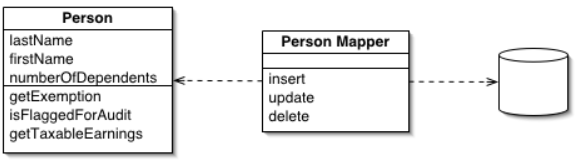
\includegraphics[scale = 0.6]{Imm/databaseMapperSketch.png}
    \caption{Esempio di UML di data mapper, dove si nota la separazione della classe dai metodi dedicati alla persistenza (nel mapper).}
\end{figure}
Framework moderni implementano questo tipo di pattern (che offre la parte di mapping senza doverli implementare ,a solo configurare). 
\subsection{Ulteriori pattern ORM}
L'aspetto del mapping è solamente una piccola parte del intero procedimento, questo perché si hanno altri problemi da dover risolvere e in generale, assocciati ai problemi, si hanno dei pattern di comportamento per risolverli. Possiamo fare una distinzione dei pattern in Comportamentali e Strutturali.
\begin{itemize}
    \item \textbf{Comportamentali}, in questa sezione abbiamo i pattern: unit of work, identity map e lazy load.
    \item \textbf{Strutturali}, abbiamo invece: value holder, identify field, embedded value e LOB
\end{itemize} 
\subsubsection{Unit of work}
In questo caso si approfondiscono le operazioni ACID cercando di capire quando sincronizzare le informazioni \textit{in memory} con il database. Questo aspetto è importante introducendo il concetto di \textbf{business transaction} per operazioni, che dal punto di vista dell'utente, devono essere eseguite con semantica di tipo \textit{all or nothing} dove o si accettano tutte le operazioni richieste o nessuna (si pensi ad esempio alla prenotazione di un biglietto). Le business transaction vanno quindi mappate nelle \textbf{system transaction} fatte dal sistema sul database. Si hanno diverse soluzioni:
\begin{itemize}
    \item \textit{aggiornare il database ogni volta che si ha una modifica in memory (slide 25)}. In pratica business transaction e system transaction coincidono ogni volta, dall'apertura alla chiusura oppure ogni volta che l'utente modifica qualcosa si effettua una system transaction. La prima soluzione è poco pratica a causa di transazioni molto lunghe (\textit{long-lasting database transactions}) in quanto un perfetto isolamento implica gestire/servire una sola query alla volta mentre un isolamento imperfetto implica che si hanno transazioni che leggono dati non definitivi, comportando inconsistenze. L'utente può aprire la transazione e restarci minuti, questo comporta anche un peggioramento delle performance del database perché blocco altre operazioni.
    \item \textit{Aggioranre il database ad ogni operazione (slide 26)}. Invece di aggiornare il database una volta sola per intera operazione,quindi da \textbf{begin} a \textbf{commit}, eseguo un aggiornamento per ogni operazione eseguita. Con il secondo caso si rischia di non poter implementare l'atomicità delle transazioni di business, che se in un certo momento fallisce non impedisce alle vecchie modifiche di essere già scritte, rompendo la \textit{all or nothing}, avendo molte difficoltà nel fare gli \textit{undo}
    \item \textit{tracciare le operazioni (nella transazione di business) e attuare tutte le modifiche in una singola transazione di sistema (slide 27)}. Tutte le operazioni sul sistema si eseguono alla fine. Il software tiene memoria di tutte le operazioni svolte dall'utente, e solamente alla fine viene avvita una transazione coin il database, in questo modo vengono eseguite tutte le notifiche al database. 
\end{itemize}
La unit of work quindi traccia ogni cambiamento (coi metodi \textit{register}) e lo attuta in una singola system transaction finale (con il \textit{commit}). Per fare questo incapsula ogni update/insert/delete, mantenendo l'integrità del database ed evitando deadlock.\\ 
A proposito di locking si ha che due business transaction possono essere attive nello stesso momento e bisogna capire come devono lavorare sul database. In questo caso si hanno due strategie:
\begin{itemize}
    \item \textbf{optimistic locking}, usato quando si hanno poche probabilità di generare conflitti, avendo diversi utenti che lavorano spesso su dati differenti, e si bassa su un numero che identifica la versione degli oggetti registrati. L'ottimismo di non avere più persone che lavorano sugli stessi dati, si traduce in record che non vengono bloccati, quindi le business transaction possono quindi interferire accedendo e modificando i record ma si sfrutta, un elemento salvato nel database, ovvero il numero di versione per tenere traccia delle modifiche. Se una transazione vede che il numero di versione di un record è incrementato significa che qualcun altro ha fatto una modifica dopo che la business transaction ha caricato l'oggetto, c'è quindi stato una modifica concorrente. In  tal caso si ricarica il record tramite un rollback e iniziamo da capo.
    Esempio di diagramma di sequenza:
    \begin{figure}[H]
        \centering
        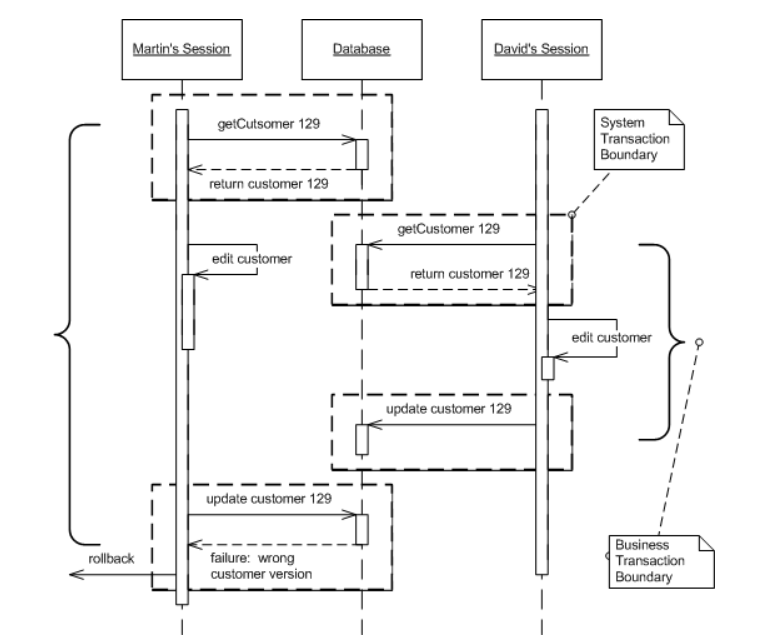
\includegraphics[scale = 0.5]{Imm/OptimisticSketch.png}
    \end{figure}
    \item \textbf{pessimistic locking}, usato quando hanno alte probabilità di generare conflitti. Gli oggetti sono bloccati non appena vengono usati riducendo la concorrenza. Non si permette quindi alle transazioni di lavorare concorrentemente riducendo però le prestazioni del sistema ma aumentando la sicurezza. Esempio di diagramma di sequenza:
    \begin{figure}[H]
        \centering
        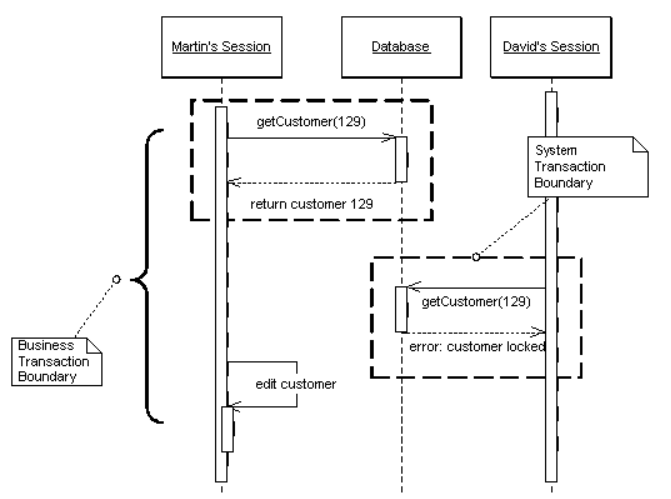
\includegraphics[scale = 0.5]{Imm/PessimisticSketch.png}
    \end{figure}
\end{itemize}
Poi, per avvisare la unit of work che un'operazione  deve essere eseguita, si hanno due pattern:
\begin{itemize}
    \item \textbf{caller registration}, dove chi modifica l'entità lo notifica direttamente alla unit of work. Questa soluzione è rischiosa in quanto il programmatore potrebbe dimenticarsi di notificare la UoW, ma permette maggior flessibilità, permettendo di decidere dinamicamente se i cambiamenti devono riflettersi sullo storage persistente. 
    \item \textbf{object registration}, dove è l'entità modificata a notificare la unit of work, che però deve obbligatoriamente avere accesso globale. Ogni cambiamento viene comunque notificato. Solitamente si usa questa soluzione ma nella variante in cui le classi persistenti non includono il codice per la notifica ma tramite una strumentazione automatica e trasparente offerta dai framework.
\end{itemize}
\subsubsection{Identity map}
In questo caso si studia il load di un'istanza direttamente a partire dal database. Se un certo record viene richiesto due volte si generano due oggetti uguali (esempio prima chiedo lo \textit{user1} e poi tutti gli \textit{user} (che ipotizziamo siano \textit{user1 \textnormal{e} user2}), avendo alla fine due copie istanziate di \textit{user1}). In pratica uno stesso oggetto può essere caricato più volte, o da azioni differenti dello stesso utente (rischiando inconsistenze, se una istanza viene modificata, oltre ad avere ridondanza di dati) o da utenti diversi (in questo spesso è intenzionale).\\ \textbf{Identity map} è quindi un oggetto con la responsabilità di identificare gli oggetti caricati in una sessione, funzionando come una sorta di cache, controllando l'eventuale presenza dell'oggetto ``in cache'' (anche se non si ha una vera cache) prima di caricarne uno nuovo (se già presente si ritorna un riferimento all'oggetto). Identity map quindi mantiene i riferimenti agli oggetti tramite un sistema chiave-valore.\\
\begin{figure}[H]
        \centering
        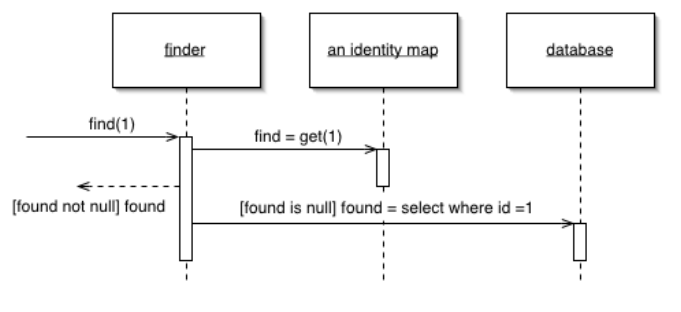
\includegraphics[scale = 0.5]{Imm/i-map.PNG}
    \end{figure}
Generalmente la chiave della mappa è quella primaria del database. Si hanno delle identity map in base al contesto di utilizzo:
\begin{itemize}
  \item una per applicazione, solo se le chiavi di entità differenti sono disgiunte
  \item una per classe, è l'opzione di default
  \item una per tabella, generalmente meglio se una per classe
\end{itemize}
La mappa è sempre accessibile.\\
\subsubsection{Lazy load}
A volte è necessario avere solo una parte di un oggetto per eseguire una certa operazione anche perché alcuni attributi (collection, bitmaps, grafi) possono essere particolarmente pesanti. Si parla quindi di efficienza.\\ 
Si procede quindi con il pattern \textbf{lazy load} che non carica i valori per alcuni attributi delle classi e caricarle solamente \textit{on-demand}, ovvero solamente se l'applicazione cerca di accedervi.\\ \textit{si aggiunge: } \textbf{Lazy load} quando crea oggetti inizializza solo alcuni attributi, evitando spesso quelli più pesanti e quelli che meno si usano, lasciando comunque possibilità si caricare in seguito ulteriori attributi non ancora inizializzati se ce ne fosse necessità, in modo \textit{on-demand}, tramite i \textit{finder}.\\ 

\subsubsection{Value holder}
Con questa tecnica si usa un oggetto, il \textbf{value holder}, come uno storage intermediario per un attributo. Anche in questo caso si ha un'inizializzazione lazy, infatti l'oggetto usato in questione, in base al caso d'uso potrebbe essere istanziato con diverse strategie di load. Si separa la logica di dominio da quella lazy di loading.\\

\subsubsection{Identify field}
Normalmente si hanno: l'identità in memory rappresentata dalla reference dell'oggetto e l'identità nel database rappresentata dalla chiave primaria. Per le quali si ha bisogno di accoppiare/sincronizzare le due identità per la consistenza dei dati.\\ 
La soluzione è usare l'\textbf{identity field} ovvero un nuovo attributo (campo) nell'oggetto il cui valore diventa la chiave primaria (solitamente chiamato \texttt{id}, di tipo \texttt{long}). Non si usano i normali attributi/identificatori della classe perché potrebbero modificare nel tempo di sviluppo del programma.\\
Si hanno infatti due tipi di chiave:
\begin{itemize}
  \item una chiave derivata da attributi dell'oggetto (che sono usati anche dall'applicazione, ad esempio la matricola). Si ha comunque rischio di duplicazione, possibile assenza di valore e cambiamenti sulla logica di dominio che impattano su quella di persistenza
  \item chiavi dedicate, sia semplici (un solo attributi) che composte (di più attributi), avendo una chiave per tabella e una per database. Nella pratica spesso hanno tipo \texttt{long} che ben supporta il check di uguaglianza (\texttt{==}) e la generazione di nuove chiavi
\end{itemize}
Si hanno varie strategie per la generazione delle chiavi:
\begin{itemize}
  \item direttamente dal database (con sequenze o id delle colonne)
  \item tramite \textit{GUID}, ovvero Globally Unique IDentifier, tramite opportuni software e libreria
  \item dall'applicazione, principalmente in due modi:
  \begin{itemize}
    \item \textit{table scan}, usando una query SQL per determinare il valore della prossima chiave
    \item \textit{key table}, usando tabelle speciali con il nome delle altre tabelle e il valore successivo della chiave
  \end{itemize}
\end{itemize}
I moderni framework ORM supportano i vari design pattern appena discussi e quelli mancanti, relativi a chiavi esterne, cascading, ereditarietà. \\ In ogni caso i pattern appena discussi sono tutti supportati dai moderni framework ORM.

\subsubsection{Embedded value}
Con questo pattern si hanno semplici oggetti, senza un chiaro concetto di identità, che possono essere inclusi in oggetti che fungono da alter-ego delle tabelle anziché creare tabelle dedicate.

\subsubsection{LOB}
Vediamo ora il pattern \textbf{Serialized Large Object (\textit{LOB})} che consiste in un grafo di oggetti memorizzati del database tramite serializzazione.\\
Questo pattern è comodo finché il LOB può essere gestito come un \textit{embedded value} ma si hanno problemi se vengono usati attributi serializzati nelle query o se il grafo ha dipendenze con oggetti non serializzati.\\ 
Si ha \textbf{Binary LOB (\textit{BLOB})}, semplice da implementare (ad esempio con \textit{Java serialization}) e compatto. Purtroppo si ha che un BLOB non è stampabile e si ha che il database deve supportare tipi binari. Crea anche problemi con il versioning delle classi.\\ 
Si ha anche \textbf{Character BLOB (CLOB)}, ad esempio tramite \textit{XML}, che però richiede librerie per il parsing e non è compatto, anche se stampabile e supportato generalmente dai database

\section{JPA 2.0}
Noi troviamo all'interno dei framework i metodi e i vari meccanismi implementati, noi dobbiamo fruire di quest'ultimi in modo dichiarativo, ovvero dobbiamo solamente andare a dire come quel meccanismo/pattern deve comportasi.
Le \textbf{Java Persistence API (\textit{JPA})}, sono un framework per il linguaggio di programmazione Java che si occupa della gestione della persistenza dei dati di un database MS relazionale nelle applicazioni.\\ 
Si ha quindi un grande set di pattern già implementati che usiamo in modo dichiarativo specificando il mapping tra enità di dominio e database. Si hanno varie implementazioni di JPA con ORM (tramite annotations e services, per comandare operazioni di persistenza), tra cui \textit{Hibernate}.\\

Una JPA Application è una normale applicazione Java dove abbiamo un insieme di classi, che implementano la business logic, e tra queste si identificano le \textit{Entity Class} (classi contenente i dati che vengono mappati sul database). Oltre a queste classi, che definiamo essere sincronizzate con il database, abbiamo anche che le nostre classi interagiscono con un servizio, il \textit{Entity manager}. Entity manager è il servizio che implementa la maggior parte dei design pattern per ORM mapping e al quale noi chiediamo di fare delle operazioni sui oggetti della classe stessa. Volendo il database può essere generato automaticamente dalle Entity Class o viceversa.

\subsection{Entity Manager}
Entity class che prendono anche il nome di \textbf{Plain Old Java Objects (\textit{POJO})}, inoltre gli oggetti che vengono creati tramite il \texttt{new} e che sono oggetti regolari fino a che non interagiscono con l'\textbf{Entity Manager} (sono normali classi con annotazioni).\\ 
Un'entità in memoria può essere in due stati:
\begin{itemize}
    \item \textbf{managed/attached}, se l'entità è sotto gestione dell'Entity Manager. Tramite tale interazione con l'Entity Manager le entità sono memorizzate nell'\textit{identity map} ed eventuali cambiamenti sono tracciati dalla \textit{unit of work}. Implementando la unit of work, può essere comandato per essere scaricare sul databse, in determinati momenti ben precisi, tutte le modifiche che sono state accumulate. D'altro canto create/remove sono responsabilità dello sviluppatore mentre le update sono rilevate automaticamente dall'Entity Manager.
    \item \textbf{unmanaged/detached}, se l'entità non è sotto gestione dell'Entity Manager, che non sa che esiste quell'entità
\end{itemize}
Posso spostare esplicitamente un oggetto da uno stato all'altro in quanto può essere utile avere oggetti unmanaged, spesso in caso di applicazioni distrubuite durante l'invio ad un altro nodo (diciamo che sono situazioni obbligate dalla pratica). Normalmente un oggetto managed rimane tale.
Si ha quindi uno schema del tipo:
\begin{figure}[H]
    \centering
    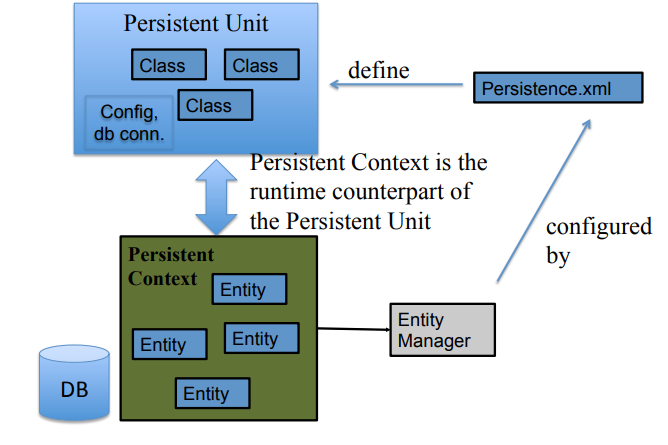
\includegraphics[scale = 0.57]{Imm/entity-manager.PNG}
\end{figure}
Nello schema si ha in alto la parte di configurazione e in basso quella di runtime. Le classi sono divise in varie \textbf{persistent unit}, ciascuna che può lavorare con un database diverso. \\ 
L'Entity Manager, che è servizio runtime con cui l'applicazione interagisce, legge il suo \textit{persistence.xml} e solamente ora sa come devono essere gestite le entità e su quale database deve mantenere la persistenza.\\

Il file \texttt{persistence.xml} è contenuto nella cartella \texttt{META-INF} del progetto e gestisce tutte le varie configurazioni. Sono indicate nel file le classi della \textit{persistent unit}: ovvero tutte le classi di entità nel progetto java (con il tag \texttt{<class>}) o contenute in un jar (con il tag \texttt{<jar-file>}).\\

In merito al mapping tra classi e database si ha che esso è definito tramite annotazioni nelle classi e all'interno dei file XML intenti a ricoprire il l'orm-mapping. I fil XML devono essere specificati all'interno del \texttt{persistence.xml} tramite il tag \texttt{<mapping-file>}.\\ 
\textbf{Nelle query si usano comunque i nomi degli oggetti}.\\
\textit{Fa un esempio di JPA completo in JAVA, seguito, ma niente di $>>$}

\subsection{Mapping}
Abbiamo diversi tipologie di mapping. Ricordiamo che indichiamo con \textit{@Entity} la nostra POJO.
\begin{itemize}
    \item \textbf{Mapping to Tables}, si identifica la classe in questione, ovvero la nostra Entity, e la si mappa con la tabella del database. Per farlo si aggiunge la notazione \textit{@Table(name="NomeTabellaDb")}. In seguito ogni attributo della classe può essere mappato come colonna della tabella attraverso \textit{@Column(name="NomeColonna")}
    \item \textbf{Simple Primary Key}, si riferisce al metodo di generazione di una chiave primaria (solitamente l'id, che spesso si trova essere di tipo Long) semplice. Alla entity va specificato che verrà utilizzato un sequenza generatrice dipendente dal DB (\textit{@SequenceGenerator}), e in seguito si specifica che la generazione è obbligatoria (\textit{@GeneratedValue}) indicando in base a quale criterio eseguire la generazione (strategy=GenerationType.Strategia, generator=“Criterio”).  
    \item \textbf{Una entità due tabelle}, come visto nel caso di \textit{Mapping to Tables}, avevamo che una tabella veniva rappresentata come singola Entity, in questo caso invece la Entity è rappresentata da due tabelle, e due tabelle sono mappate da una sola Entity. Per mappare una seconda tabella nella Entity usiamo \textit{@SecondaryTable(name=“Tabella2”, pkJoinColumns={@PrimaryKeyJoinColum(name=“PK2Tab”)})}
\end{itemize}

Possiamo anche andare a dichiarare che un determinato attributo di una certa Entity è incorporabile. Ci serve solamente specificare che la classe da incorporare sia annotata con \textit{@Embeddable}, e nella Entity usare la \textit{@Embedded} notazione per poi andare a utilizzarla.\\

Possiamo inoltre aggiungere che le chiavi primarie utilizzano la notazione \textit{Long} per via dell'efficienza che comporta avere valori di tipo Long nei confronti di uguaglianza. \\

\subsection{Refernce tra Entity diverse}
Segue lo stesso concetto del linguaggio SQL:
\begin{itemize} 
    \item \textit{One-to-One} monodirezionale, la chiave primaria \textit{a} della tabella \textit{A} è anche chiave esterna referenziata da una colonna \textit{b} della tabella \textit{B}. Ricordiamo che ogni tabella è rappresentata da una singola Entity nel JPA.
    \item \textit{One-to-One} bidirezionale, segue lo stesso principio della mono, con la particolarità che possiamo tenere traccia attraverso \textit{mappedBy} per capire quale Entity ha eseguito il mapping. Quindi per entrambe le Entity abbiamo un reference per la Entity in relazione. 
    \item \textit{One-to-Many}, vengono create delle collezioni di dati. I dati vengono ritornati dalle operazioni di Join tra le tabelle in relazione.\textit{Una Entity può avere collegate più record di un attributo di una seconda Entity}
    \item \textit{One-to-Many} bidirezionale, vengono sempre create delle collezioni di dati, da una parte abbiamo una relazione \textit{Many-to-One}, nell'altra entity invece abbiamo una \textit{One-to-many} per la collezione dati di cui si parlava prima. 
    \item \textit{Many-to-One}, usa il metodo inverso utilizzato dalla One-to-Many. 
    \item \textit{Many-to-Many}
\end{itemize}

\subsection{Mapping Hierachies}
Nella OOP posso avere gerarchie tra gli oggetti ed ereditarietà ma questi concetti non si hanno nei database e quindi serve un mapping dedicato per eseguire query che sfruttano le gerarchie. Il mapping deve essere esplicitamente specificata.\\ Si hanno tre strategie per il mapping (\textbf{su slide esempi delle varie annotazioni per Java}):
\begin{enumerate}
      \item \textbf{single table}, che prevede una tabella per ogni classe in rapporto di gerarchia tra loro. Si ha quindi una colonna che deve rappresentare il tipo di oggetto (per distinguere le varie classi) di tipo stringa. È un metodo facile da implementare e veloce ma obbliga ad avere tabelle che possono contenere valori NULL (una classe derivata ha attributi in più di quella orinale e diversi da un'altra classe derivata dalla stessa classe originale etc$\ldots$). Si ha comunque uno spreco di risorse.
      \item \textbf{one table per concrete class}, dove ogni classe (sia padre che figli) hanno una tavella associata con un campo per ogni attributo (per le figlie anche quelli ereditati). Tutti gli attributi di una classe sono quindi in una singola tabella dedicata. Si ha un maggior controllo dei vincoli e un mapping ancora semplice ma è difficile da gestire con l'Entity Manager e il databaseMS deve supportare la \textit{SQL UNION}
      \item \textbf{one table per subclass} dove si ha una classe per tabella ma senza ricopia degli attributi per le classi figlie (che sono caratterizzate solo dall'id e dagli attributi extra rispetto alla classe padre). Si ha quindi un mapping ``uno a uno''. Questa strategia supporta i vincoli tabellari e non richiede la \textit{SQL UNION} ma si ha un istanza ``splittata'' su più tabelle ed è generalmente una soluzione lenta in esecuzione (dovendo eseguire i \textit{join})
\end{enumerate}